\documentclass{standalone}
\usepackage{tikz}
\usetikzlibrary{patterns, positioning}


\begin{document}
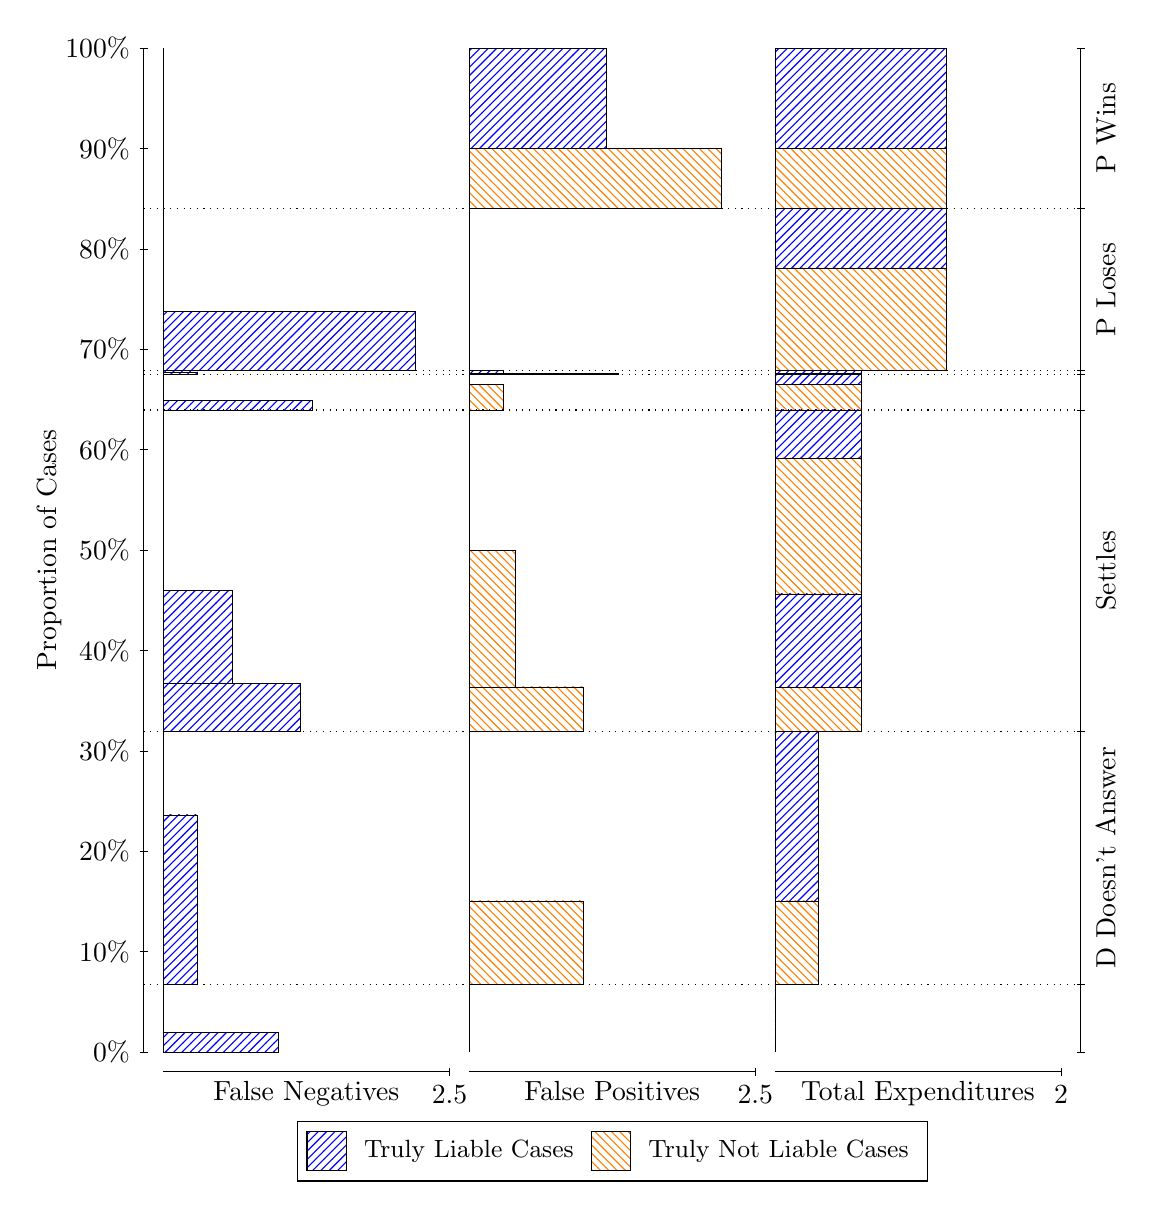
\begin{tikzpicture}
\draw[black, very thin] (1.5,1.75) -- (1.5,14.5);
\node[rotate=90, text=black, anchor=center] at (0.3, 8.125) {Proportion of Cases};
\draw[black, very thin] (1.45,1.75) -- (1.55,1.75);
\node[text=black, anchor=east] at (1.45, 1.75) {0\%};
\draw[black, very thin] (1.45,3.025) -- (1.55,3.025);
\node[text=black, anchor=east] at (1.45, 3.025) {10\%};
\draw[black, very thin] (1.45,4.3) -- (1.55,4.3);
\node[text=black, anchor=east] at (1.45, 4.3) {20\%};
\draw[black, very thin] (1.45,5.575) -- (1.55,5.575);
\node[text=black, anchor=east] at (1.45, 5.575) {30\%};
\draw[black, very thin] (1.45,6.85) -- (1.55,6.85);
\node[text=black, anchor=east] at (1.45, 6.85) {40\%};
\draw[black, very thin] (1.45,8.125) -- (1.55,8.125);
\node[text=black, anchor=east] at (1.45, 8.125) {50\%};
\draw[black, very thin] (1.45,9.4) -- (1.55,9.4);
\node[text=black, anchor=east] at (1.45, 9.4) {60\%};
\draw[black, very thin] (1.45,10.675) -- (1.55,10.675);
\node[text=black, anchor=east] at (1.45, 10.675) {70\%};
\draw[black, very thin] (1.45,11.95) -- (1.55,11.95);
\node[text=black, anchor=east] at (1.45, 11.95) {80\%};
\draw[black, very thin] (1.45,13.225) -- (1.55,13.225);
\node[text=black, anchor=east] at (1.45, 13.225) {90\%};
\draw[black, very thin] (1.45,14.5) -- (1.55,14.5);
\node[text=black, anchor=east] at (1.45, 14.5) {100\%};

\draw[black, very thin] (13.4,1.75) -- (13.4,14.5);
\draw[black, very thin] (13.35,1.75) -- (13.45,1.75);
\node[anchor=west] at (13.35, 1.75) {};
\draw[black, very thin] (13.35,2.6057) -- (13.45,2.6057);
\node[anchor=west] at (13.35, 2.6057) {};
\draw[black, very thin] (13.35,5.8242) -- (13.45,5.8242);
\node[anchor=west] at (13.35, 5.8242) {};
\draw[black, very thin] (13.35,9.9033) -- (13.45,9.9033);
\node[anchor=west] at (13.35, 9.9033) {};
\draw[black, very thin] (13.35,10.354) -- (13.45,10.354);
\node[anchor=west] at (13.35, 10.354) {};
\draw[black, very thin] (13.35,10.402) -- (13.45,10.402);
\node[anchor=west] at (13.35, 10.402) {};
\draw[black, very thin] (13.35,12.463) -- (13.45,12.463);
\node[anchor=west] at (13.35, 12.463) {};
\draw[black, very thin] (13.35,14.5) -- (13.45,14.5);
\node[anchor=west] at (13.35, 14.5) {};

\draw[black, very thin, pattern color=blue, pattern=north east lines] (1.75,1.75) rectangle (3.2033,1.9966);
\draw[black, very thin, pattern color=orange, pattern=north west lines] (1.75,1.9966) rectangle (1.75,2.6057);
\draw[black, very thin, pattern color=blue, pattern=north east lines] (1.75,2.6057) rectangle (2.186,4.7614);
\draw[black, very thin, pattern color=orange, pattern=north west lines] (1.75,4.7614) rectangle (1.75,5.8242);
\draw[black, very thin, pattern color=blue, pattern=north east lines] (1.75,5.8242) rectangle (3.494,6.4333);
\draw[black, very thin, pattern color=blue, pattern=north east lines] (1.75,6.4333) rectangle (2.622,7.6121);
\draw[black, very thin, pattern color=orange, pattern=north west lines] (1.75,7.6121) rectangle (1.75,9.9033);
\draw[black, very thin, pattern color=blue, pattern=north east lines] (1.75,9.9033) rectangle (3.6393,10.029);
\draw[black, very thin, pattern color=orange, pattern=north west lines] (1.75,10.029) rectangle (1.75,10.354);
\draw[black, very thin, pattern color=blue, pattern=north east lines] (1.75,10.354) rectangle (2.186,10.388);
\draw[black, very thin, pattern color=orange, pattern=north west lines] (1.75,10.388) rectangle (1.75,10.402);
\draw[black, very thin, pattern color=blue, pattern=north east lines] (1.75,10.402) rectangle (4.9473,11.157);
\draw[black, very thin, pattern color=orange, pattern=north west lines] (1.75,11.157) rectangle (1.75,12.463);
\draw[black, very thin, pattern color=orange, pattern=north west lines] (1.75,12.463) rectangle (1.75,13.229);
\draw[black, very thin, pattern color=blue, pattern=north east lines] (1.75,13.229) rectangle (1.75,14.5);
\draw[black, very thin, pattern color=orange, pattern=north west lines] (5.6333,1.75) rectangle (5.6333,2.3592);
\draw[black, very thin, pattern color=blue, pattern=north east lines] (5.6333,2.3592) rectangle (5.6333,2.6057);
\draw[black, very thin, pattern color=orange, pattern=north west lines] (5.6333,2.6057) rectangle (7.0867,3.6685);
\draw[black, very thin, pattern color=blue, pattern=north east lines] (5.6333,3.6685) rectangle (5.6333,5.8242);
\draw[black, very thin, pattern color=orange, pattern=north west lines] (5.6333,5.8242) rectangle (7.0867,6.3878);
\draw[black, very thin, pattern color=orange, pattern=north west lines] (5.6333,6.3878) rectangle (6.2147,8.1155);
\draw[black, very thin, pattern color=blue, pattern=north east lines] (5.6333,8.1155) rectangle (5.6333,9.9033);
\draw[black, very thin, pattern color=orange, pattern=north west lines] (5.6333,9.9033) rectangle (6.0693,10.229);
\draw[black, very thin, pattern color=blue, pattern=north east lines] (5.6333,10.229) rectangle (5.6333,10.354);
\draw[black, very thin, pattern color=orange, pattern=north west lines] (5.6333,10.354) rectangle (7.5227,10.369);
\draw[black, very thin, pattern color=blue, pattern=north east lines] (5.6333,10.369) rectangle (6.0693,10.402);
\draw[black, very thin, pattern color=orange, pattern=north west lines] (5.6333,10.402) rectangle (5.6333,11.709);
\draw[black, very thin, pattern color=blue, pattern=north east lines] (5.6333,11.709) rectangle (5.6333,12.463);
\draw[black, very thin, pattern color=orange, pattern=north west lines] (5.6333,12.463) rectangle (8.8307,13.229);
\draw[black, very thin, pattern color=blue, pattern=north east lines] (5.6333,13.229) rectangle (7.3773,14.5);
\draw[black, very thin, pattern color=orange, pattern=north west lines] (9.5167,1.75) rectangle (9.5167,2.3592);
\draw[black, very thin, pattern color=blue, pattern=north east lines] (9.5167,2.3592) rectangle (9.5167,2.6057);
\draw[black, very thin, pattern color=orange, pattern=north west lines] (9.5167,2.6057) rectangle (10.062,3.6685);
\draw[black, very thin, pattern color=blue, pattern=north east lines] (9.5167,3.6685) rectangle (10.062,5.8242);
\draw[black, very thin, pattern color=orange, pattern=north west lines] (9.5167,5.8242) rectangle (10.607,6.3878);
\draw[black, very thin, pattern color=blue, pattern=north east lines] (9.5167,6.3878) rectangle (10.607,7.5665);
\draw[black, very thin, pattern color=orange, pattern=north west lines] (9.5167,7.5665) rectangle (10.607,9.2942);
\draw[black, very thin, pattern color=blue, pattern=north east lines] (9.5167,9.2942) rectangle (10.607,9.9033);
\draw[black, very thin, pattern color=orange, pattern=north west lines] (9.5167,9.9033) rectangle (10.607,10.229);
\draw[black, very thin, pattern color=blue, pattern=north east lines] (9.5167,10.229) rectangle (10.607,10.354);
\draw[black, very thin, pattern color=orange, pattern=north west lines] (9.5167,10.354) rectangle (10.607,10.369);
\draw[black, very thin, pattern color=blue, pattern=north east lines] (9.5167,10.369) rectangle (10.607,10.402);
\draw[black, very thin, pattern color=orange, pattern=north west lines] (9.5167,10.402) rectangle (11.697,11.709);
\draw[black, very thin, pattern color=blue, pattern=north east lines] (9.5167,11.709) rectangle (11.697,12.463);
\draw[black, very thin, pattern color=orange, pattern=north west lines] (9.5167,12.463) rectangle (11.697,13.229);
\draw[black, very thin, pattern color=blue, pattern=north east lines] (9.5167,13.229) rectangle (11.697,14.5);
\draw[black, dotted] (1.5,2.6057) -- (13.4,2.6057);
\draw[black, dotted] (1.5,5.8242) -- (13.4,5.8242);
\draw[black, dotted] (1.5,9.9033) -- (13.4,9.9033);
\draw[black, dotted] (1.5,10.354) -- (13.4,10.354);
\draw[black, dotted] (1.5,10.402) -- (13.4,10.402);
\draw[black, dotted] (1.5,12.463) -- (13.4,12.463);
\draw[black, very thin] (1.75,1.5) -- (5.3833,1.5);
\node[text=black, anchor=north] at (3.5667, 1.5) {False Negatives};
\draw[black, very thin] (5.3833,1.45) -- (5.3833,1.55);
\node[text=black, anchor=north] at (5.3833, 1.45) {2.5};

\draw[black, very thin] (5.6333,1.5) -- (9.2667,1.5);
\node[text=black, anchor=north] at (7.45, 1.5) {False Positives};
\draw[black, very thin] (9.2667,1.45) -- (9.2667,1.55);
\node[text=black, anchor=north] at (9.2667, 1.45) {2.5};

\draw[black, very thin] (9.5167,1.5) -- (13.15,1.5);
\node[text=black, anchor=north] at (11.333, 1.5) {Total Expenditures};
\draw[black, very thin] (13.15,1.45) -- (13.15,1.55);
\node[text=black, anchor=north] at (13.15, 1.45) {2};


\node[text=black, centered, rotate=90] at (13.72, 4.215) {D Doesn't Answer};
\node[text=black, centered, rotate=90] at (13.72, 7.8638) {Settles};


\node[text=black, centered, rotate=90] at (13.72, 11.433) {P Loses};
\node[text=black, centered, rotate=90] at (13.72, 13.482) {P Wins};

\draw (7.449999999999999,1.5) node[draw=none] (baseCoordinate) {};
\begin{scope}[align=center]
        \matrix[scale=0.5, draw=black, below=0.5cm of baseCoordinate, nodes={draw}, column sep=0.1cm]{
            \node[rectangle, draw, minimum width=0.5cm, minimum height=0.5cm, pattern color=blue, pattern=north east lines] {}; &
            \node[draw=none, font=\small, text=black] (B) {Truly Liable Cases}; &
            \node[rectangle, draw, minimum width=0.5cm, minimum height=0.5cm, pattern color=orange, pattern=north west lines] {}; &
            \node[draw=none, font=\small, text=black] (B) {Truly Not Liable Cases}; \\
            };
\end{scope}

\end{tikzpicture}
\end{document}